\section{Data Acquisition}
\label{sec:dataset}

\subsection{Acquisition and composition}
The \textsc{CrackID} frozen benchmark snapshot holds 140 photographs of 17 exterior walls at one site over four half-days (two consumer handsets; archived at Mendeley Data). Walls span stippled render (textured) and smooth painted plaster (often crack-only in frame). Split: 6 validation walls wall01--wall06 (66 photos, 66 identities) and 11 test walls wall07--wall17 (74 photos, 146 identities); only identities in ${\geq}2$ photos yield answerable queries (18 val, 19 test; $n_Q{=}280$ test, $439$ val). Two walls added later (wall18--wall19) are excluded from every number in this paper. Each wall is one continuous walk-around (median $3$\,s between consecutive frames, max span $81$\,s), so the data measures within-visit viewpoint/scale correspondence, a hypothesized upper bound on multi-visit performance.

\smallskip
\noindent\emph{Adjacent-frame retrieval.} $100\%$ of $280$ answerable test queries are answered by the adjacent frame; Sec.~\ref{sec:results} gap sweeps ($280{\to}205{\to}149{\to}105$ for gaps $0{\to}3$) find flat Rank-1 on a shrinking pool, characterising short-baseline robustness rather than proving irrelevance.

\subsection{Annotation, and why it needs auditing}
\label{sec:annotation}
One click per crack is propagated across consecutive frames via ORB homography plus one-to-one assignment, then fragment merges join components of one physical crack. Merge risk concentrates here: a wrong join turns a hard negative into a free positive for \emph{every} method. We report extent, not correctness: $95/212$ identities ($45\%$; $70/146$, $48\%$ on test) come from merges, with median bridged gaps of $228$\,px (test) and $286$\,px (val). A single annotator validated all clicks with full triage of unclaimed points ($107/1\,023$ naming no crack; full counts in supplement); agreement is unmeasured, so merge risk is bounded by reporting, not removed. Counts refer to the frozen snapshot (Table~\ref{tab:units}); the live \texttt{dataset/labels/} has since been re-edited (wall18--wall19 added, changelog rebuilt without gap fields) and no longer reproduces these counts until the benchmark is re-run.
\begin{figure}[t]
\centering
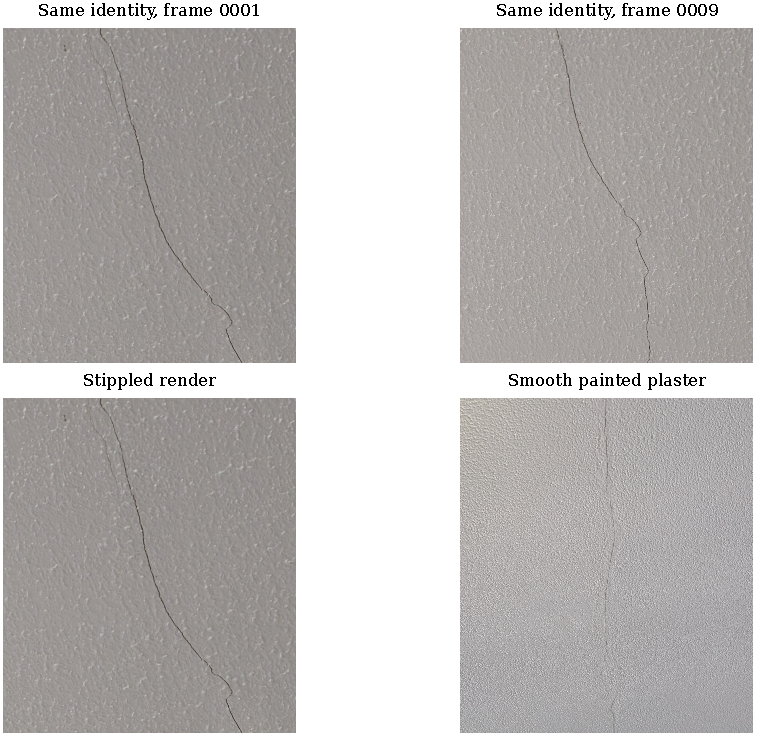
\includegraphics[width=0.85\columnwidth]{figs/dataset_examples.pdf}
\caption{Real \textsc{CrackID} captures. Top: one identity in non-adjacent frames. Bottom: stippled render vs smooth plaster. Labels use homography propagation; illustrative, not an independent audit.}
\label{fig:dataset-examples}
\end{figure}
